\documentclass[convert={density=1024}]{standalone}
\usepackage{amsmath, amsthm, amsfonts}
\usepackage{tikz-cd, kotex}
\usepackage{../../preamble/quiver}
\usepackage{../../preamble/Math-operators}
\begin{document}

% Exponential map (Lie_correspondence-1.png)
\begin{tikzcd}
	G & H \\
	{\mathfrak{g}} & {\mathfrak{h}}
	\arrow["F", from=1-1, to=1-2]
	\arrow["\exp"', from=2-2, to=1-2]
	\arrow["\exp", from=2-1, to=1-1]
	\arrow["dF"', from=2-1, to=2-2]
\end{tikzcd}

\end{document}

% Quotient_map (Examples_of_manifolds-2.png)
\begin{tikzcd}
	{\widetilde{U}_i} \\
	{U_i} & {\mathbb{R}^n}
	\arrow["{\varphi_i}"', from=2-1, to=2-2]
	\arrow["{\pi\vert_{\widetilde{U}_i}}"', from=1-1, to=2-1]
	\arrow[dashed, from=1-1, to=2-2]
\end{tikzcd}

% Differential (Differentials-2.png)
\begin{tikzcd}
	{\mathcal{C}^\infty_{N,F(p)}} & {\mathcal{C}_{M,p}^\infty} \\
	& {\mathbb{R}}
	\arrow["{F^\ast}", from=1-1, to=1-2]
	\arrow[""{name=0, anchor=center, inner sep=0}, "{L\in(\mathcal{C}_{M,p}^\infty)^\ast}", from=1-2, to=2-2]
	\arrow[""{name=1, anchor=center, inner sep=0}, "{{({F^\ast})^\ast}(L)=L\circ F^\ast\in(\mathcal{C}^\infty_{N, F(p)})^\ast}"', dashed, from=1-1, to=2-2]
	\arrow[shift right=1, shorten <=3pt, shorten >=3pt, Rightarrow, from=0, to=1]
\end{tikzcd}

% Tangent_space_of_vector_space (Examples_of_differentials-1.png)
\begin{tikzcd}
	V & W \\
	{T_xV} & {T_{L(x)}W}
	\arrow[Rightarrow, no head, from=1-1, to=2-1]
	\arrow["L", from=1-1, to=1-2]
	\arrow[Rightarrow, no head, from=1-2, to=2-2]
	\arrow["{dL_x}"', from=2-1, to=2-2]
\end{tikzcd}

% Immersion and embedding (Submanifolds-1.png)
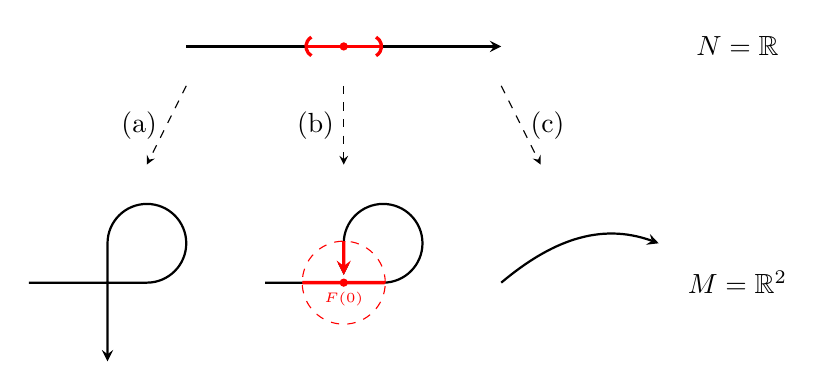
\begin{tikzpicture}
	\draw[thick, -{stealth}] (-2,0)--(2,0);
	\draw[very thick, red, Parenthesis-Parenthesis] (-.5,0)--(.5,0);
	\fill[red] (0,0) circle[radius=1.5pt];
	\draw[thick, -{stealth}] (-4,-3)--(-2.5,-3) arc (-90:180:.5)--(-3,-4);
	\draw[thick, -{stealth}] (-1,-3)--(0.5,-3) arc (-90:180:.5)--(0,-2.9);
	\draw[thick, -{stealth}] (2,-3) to[out=40, in=160] (4,-2.5);
	\draw[dashed, -{stealth}] (-2,-0.5)--(-2.5,-1.5) node[midway, left]{(a)};
	\draw[dashed, -{stealth}] (0,-0.5)--(0,-1.5) node[midway, left]{(b)};
	\draw[dashed, -{stealth}] (2,-0.5)--(2.5,-1.5) node[midway, right]{(c)};
	\draw[dashed, red] (0,-3) circle[radius=15pt];
	\begin{scope}
		\clip (0,-3) circle[radius=15pt];
		\fill[red] (0,-3) circle[radius=1.5pt] node[below]{\tiny $F(0)$};
		\draw[red, very thick, -{stealth}] (-1,-3)--(0.5,-3) arc (-90:180:.5)--(0,-2.9);
    \end{scope}
    \draw (5,0) node{$N=\mathbb{R}$};
    \draw (5,-3) node{$M=\mathbb{R}^2$};
\end{tikzpicture}

% Counterexample_1 (Uniqueness_of_submanifold-1.png)
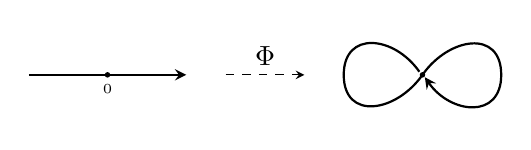
\begin{tikzpicture}
	\draw[thick, -{stealth}] (-5,0)--(-3,0);
	\fill (-4,0) circle[radius=1pt] node[below]{\tiny $0$};
	\draw[dashed, -{stealth}] (-2.5,0)--(-1.5,0) node[midway, above]{$\Phi$};
	\draw[thick] (0,0) to[out=55, in=90, looseness=1.5] (1,0);
	\draw[thick, -{stealth}] (1,0) to[out=-90, in=-55, looseness=1.5] (0.03,-0.03);
	\draw[thick] (-.04,.04) to[out=125, in=90, looseness=1.5] (-1,0);
	\draw[thick] (-1,0) to[out=-90, in=-125, looseness=1.5] (0,0);
	\fill (0,0) circle[radius=1pt];
\end{tikzpicture}

% Counterexample_2 (Uniqueness_of_submanifold-2.png)
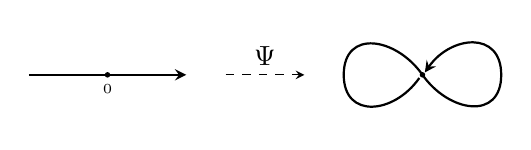
\begin{tikzpicture}
	\draw[thick, -{stealth}] (-5,0)--(-3,0);
	\fill (-4,0) circle[radius=1pt] node[below]{\tiny $0$};
	\draw[dashed, -{stealth}] (-2.5,0)--(-1.5,0) node[midway, above]{$\Psi$};
	\draw[thick, {stealth}-] (0.03,0.03) to[out=55, in=90, looseness=1.5] (1,0);
	\draw[thick] (1,0) to[out=-90, in=-55, looseness=1.5] (0,0);
	\draw[thick] (0,0) to[out=125, in=90, looseness=1.5] (-1,0);
	\draw[thick] (-1,0) to[out=-90, in=-125, looseness=1.5] (-0.04,-0.04);
	\fill (0,0) circle[radius=1pt];
\end{tikzpicture}

% Counterexample_3 (Uniqueness_of_submanifold-3.png)
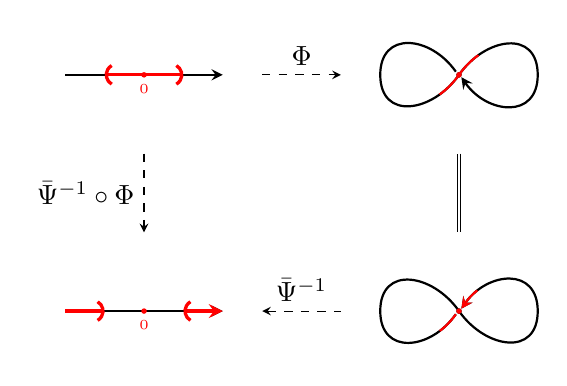
\begin{tikzpicture}
	\draw[thick, -{stealth}] (-5,0)--(-3,0);
	\draw[red, Parenthesis-Parenthesis, very thick] (-4.5,0)--(-3.5,0);
	\fill[red] (-4,0) circle[radius=1pt] node[below]{\tiny $0$};
	\draw[dashed, -{stealth}] (-2.5,0)--(-1.5,0) node[midway, above]{$\Phi$};
	\draw[thick] (0,0) to[out=55, in=90, looseness=1.5] (1,0);
	\draw[thick, -{stealth}] (1,0) to[out=-90, in=-55, looseness=1.5] (0.03,-0.03);
	\draw[thick] (-.04,.04) to[out=125, in=90, looseness=1.5] (-1,0);
	\draw[thick] (-1,0) to[out=-90, in=-125, looseness=1.5] (0,0);
	\fill (0,0) circle[radius=1pt];
	\begin{scope}
		\clip (0,0) circle[radius=10pt];
		\draw[red, thick] (0,0) to[out=55, in=90, looseness=1.5] (1,0);
		\draw[red, thick] (-1,0) to[out=-90, in=-125, looseness=1.5] (0,0);
		\fill[red] (0,0) circle[radius=1pt];
    \end{scope}
    \draw[double] (0,-1)--(0,-2);
	\draw[thick, -{stealth}] (-5,-3)--(-3,-3);
	\fill[red] (-4,-3) circle[radius=1pt] node[below]{\tiny $0$};
	\draw[dashed, {stealth}-] (-2.5,-3)--(-1.5,-3) node[midway, above]{$\bar{\Psi}^{-1}$};
	\draw[thick, {stealth}-] (0.03,-2.97) to[out=55, in=90, looseness=1.5] (1,-3);
	\draw[thick] (1,-3) to[out=-90, in=-55, looseness=1.5] (0,-3);
	\draw[thick] (0,-3) to[out=125, in=90, looseness=1.5] (-1,-3);
	\draw[thick] (-1,-3) to[out=-90, in=-125, looseness=1.5] (-0.04,-3.04);
	\fill (0,-3) circle[radius=1pt];
	\begin{scope}
		\clip (0,-3) circle[radius=10pt];
		\draw[red, thick, {stealth}-] (0.03,-2.97) to[out=55, in=90, looseness=1.5] (1,-3);
		\draw[red, thick] (-1,-3) to[out=-90, in=-125, looseness=1.5] (-0.04,-3.04);
		\fill[red] (0,-3) circle[radius=1pt];
    \end{scope}
    \draw[red, very thick, Parenthesis-{stealth}] (-3.5,-3)--(-3,-3);
    \draw[red, very thick, Parenthesis-] (-4.5,-3)--(-5,-3);
    \draw[dashed, -{stealth}] (-4,-1)--(-4,-2) node[midway, left]{$\bar{\Psi}^{-1}\circ\Phi$};
\end{tikzpicture}

% Uniqueness of submanifold structure (Uniqueness_of_submanifold-4.png)
\begin{tikzcd}
	{(A,\mathcal{T}',\mathcal{A}')} & M \\
	& {(A,\mathcal{T},\mathcal{A})}
	\arrow["{\iota'}", from=1-1, to=1-2]
	\arrow["\iota"', from=2-2, to=1-2]
	\arrow["{\operatorname{id}}"', dashed, from=1-1, to=2-2]
\end{tikzcd}

% Bundle_map (Vector_bundles-1.png)
\begin{tikzcd}
	E & {E'} \\
	B & {B'}
	\arrow[from=1-1, to=2-1]
	\arrow[from=1-1, to=1-2]
	\arrow[from=1-2, to=2-2]
	\arrow[from=2-1, to=2-2]
\end{tikzcd}

% Hom_functor (Vector_bundles-2.png)
\begin{tikzcd}
	V & W \\
	{V'} & {W'}
	\arrow[""{name=0, anchor=center, inner sep=0}, "u", from=1-1, to=1-2]
	\arrow[""{name=1, anchor=center, inner sep=0}, "{g\circ u\circ f^{-1}}"', from=2-1, to=2-2]
	\arrow["g", from=1-2, to=2-2]
	\arrow["f"', from=1-1, to=2-1]
	\arrow["{\operatorname{Hom}(f,g)}"{description}, shorten <=4pt, shorten >=4pt, Rightarrow, from=0, to=1]
\end{tikzcd}

% Chain_map_in_dR (Differential_forms-1.png)
\begin{tikzcd}
	0 & {\Omega^0(M)} & {\Omega^1(M)} & {\Omega^2(M)} & \cdots \\
	0 & {\Omega^0(N)} & {\Omega^1(N)} & {\Omega^2(N)} & \cdots
	\arrow[from=1-1, to=1-2]
	\arrow["d", from=1-2, to=1-3]
	\arrow["d", from=1-3, to=1-4]
	\arrow["d", from=1-4, to=1-5]
	\arrow[from=2-1, to=2-2]
	\arrow["d", from=2-2, to=2-3]
	\arrow["d", from=2-3, to=2-4]
	\arrow["d", from=2-4, to=2-5]
	\arrow["{F^\ast}", from=2-2, to=1-2]
	\arrow["{F^\ast}", from=2-3, to=1-3]
	\arrow["{F^\ast}", from=2-4, to=1-4]
\end{tikzcd}

% F-related_vector_fields (Lie_derivative-1.png)
\begin{tikzcd}
	M & N \\
	TM & TN
	\arrow["F", from=1-1, to=1-2]
	\arrow["dF"', from=2-1, to=2-2]
	\arrow["X"', from=1-1, to=2-1]
	\arrow["Y", from=1-2, to=2-2]
\end{tikzcd}

